\documentclass[acmtog]{techreportacmart}

\usepackage{booktabs} % For formal tables


\usepackage[ruled]{algorithm2e} % For algorithms
\renewcommand{\algorithmcfname}{ALGORITHM}
\SetAlFnt{\small}
\SetAlCapFnt{\small}
\SetAlCapNameFnt{\small}
\SetAlCapHSkip{0pt}
\IncMargin{-\parindent}

% Copyright
\setcopyright{none}

\settopmatter{printacmref=false, printccs=false, printfolios=true}
\citestyle{acmauthoryear}
\setcitestyle{square}

% Document starts
\begin{document}
% Title portion
\title{Learning Physics Constrained Dynamics Using Autoencoders} 
\author{Izabella Pavlova}
\affiliation{%
  \institution{Technical University of Munich}
}

\renewcommand\shortauthors{Pavlova}

\begin{abstract}
Multifrequency media access control has been well understood in
general wireless ad hoc networks, while in wireless sensor networks,
researchers still focus on single frequency solutions. In wireless
sensor networks, each device is typically equipped with a single
radio transceiver and applications adopt much smaller packet sizes
compared to those in general wireless ad hoc networks. Hence, the
multifrequency MAC protocols proposed for general wireless ad hoc
networks are not suitable for wireless sensor network applications,
which we further demonstrate through our simulation experiments. In
this article, we propose MMSN, which takes advantage of
multifrequency availability while, at the same time, takes into
consideration the restrictions of wireless sensor networks. Through
extensive experiments, MMSN exhibits the prominent ability to utilize
parallel transmissions among neighboring nodes. When multiple physical
frequencies are available, it also achieves increased energy
efficiency, demonstrating the ability to work against radio
interference and the tolerance to a wide range of measured time
synchronization errors.
\end{abstract}

%
% End generated code
%

\keywords{Wireless sensor networks, media access control,
multi-channel, radio interference, time synchronization}


\thanks{This report is a part of the lecture, Master-Seminar - Deep Learning in Physics, Informatics 15, Technical University of Munich.
\\
The original work is introduced by~\cite{NEURIPS2022_6d5e0357}.}
\maketitle


\section{Introduction} % problem statement
% TODO: discrete points are equally spaced in time
In addition, one may think that the estimator network can directly predict the system parameters given the input observation without taking the states. The reason to predict the states is that for some applications, it may be useful to know the state of the system. For example, for a self-driving car, we would like to know the speed of other vehicles by using observations from cameras. Knowing the speed of other vehicles (i.e., , the state) allows the self-driving car to plan for a trajectory, which is important for the safe deployment of the system. In addition, we would like to increase the interpretability of the model. The inclusion of the state allows the system designer to ensure the representation learned by neural networks is informative.
\section{Background} % physics-informed learning + koopmann
\section{ALPS Architecture}
The autoencoder with latent physics (ALPS) model (Fig.~\ref{fig:architecture}) estimates states and physical parameters of the system using four main components. Firstly, encoder ${h}$ estimates states $\tilde{x}_{s}$ from an observation sequence ${o_s}$. Secondly, estimator ${f}$ predicts physical parameters ${\theta}$  from the states $\tilde{x}_{s}$. Thirdly, using the initial state and predicted parameters ${\theta}$ physics simulator generates a state trajectory $\hat{x}_{s}$ consistent with the laws of physics. Lastly, a decoder ${g}$ reconstructs observations $\hat{o}_{s}$ from the state trajectory $\hat{x}_{s}$. The autoencoder is trained to minimize the observation reconstruction loss $\sum_{s} \lVert o_{s} - \hat{o}_{s} \rVert_{2}^{2}$. In addition, the encoder ${h}$ is trained to minimize the sum of squared state errors $\sum_{s} \lVert \tilde{x}_{s} - \hat{x}_{s} \rVert_{2}^{2}$.
\begin{figure}
  \centering
  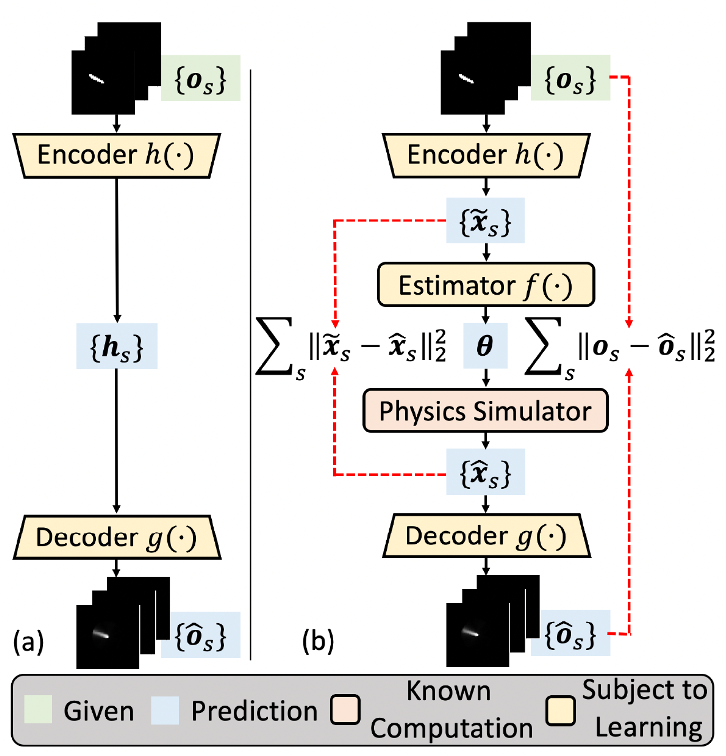
\includegraphics[width=0.4\textwidth]{architecture}
  \caption{ALPS Architecture}
  \label{fig:architecture}
\end{figure}
\textbf{The encoder network.} Depending on the type of observations — pixel images or direct measurements — a convolution or feedforward network is used to represent an observation ${o}$ as a vector embedding ${z'}$. To understand the dynamics within the data, the local and global context of the dynamics are extracted by aggregating the vector embedding ${z'}$ using a self-attention network~\cite{NIPS2017_3f5ee243}.
\\
Firstly, to incorporate positional information, a positional encoding is added to the embeddings which are then stacked over ${\tau}$ steps to form a matrix. Secondly, to calculate the attention softmax is taken over the ${\tau}$ steps. Thirdly, to allow the model to jointly attend to information from different representation subspaces at different positions the multi-head attention mechanism is applied (\ref{eq:multihead},\ref{eq:attention}).
\begin{equation}
  \label{eq:multihead}
  \text{Multihead} = \text{Concat}(\text{head}_1, \ldots, \text{head}_h) \cdot W^{O}
\end{equation}
\begin{equation}
  \label{eq:attention}
  \text{head}_i = \text{Attention}(Q, K, V) = \text{softmax}\left(\frac{{QK^T}}{\sqrt{d}}\right)V,
\end{equation}
where ${Q, K, V}$ represent the query, key, and value matrices of dimensionality ${d}$ respectively and $W^{O}$ are learnable matrices.\\
Finally, using Gaussian and Mises distributions as posterior for translational and rotational coordinates accordingly, a feedforward network produces the parameters of the distribution for each state in the sequence.
\\
\textbf{The parameter estimator network.} It was shown that multilayer perceptrons (MLPs) are affected by spectral bias~\cite{rahamanspectral} i.e.~lower frequencies are learned first. Therefore, for systems that involve periodical or vibrational behavior, such as pendulum and oscillator, the input is passed through a Fourier transform on each component ${j}$ of state trajectory~(\ref{eq:fourier}) in order to capture high frequency content in the data~\cite{tancik2020ffn}. For other systems, which do not have periodic behavior the transformation is not needed. For each Fourier feature mapping a residual network~\cite{7780459} is used to get a representation. The parameter estimator MLP network predicts physical parameters ${\theta}$ by taking a concatenation of the magnitudes of Fourier features ${|\tilde{X}_{\omega}(j)|}$ from states $\tilde{x}_{s}$.
\begin{equation}
  \label{eq:fourier}
  \tilde{X}_{\omega}(j) := \sum_{k=t-\tau+1}^{t} \tilde{x}_k(j) \left( \cos \left(\frac{2\pi}{\tau} \omega k \right) - i \cdot \sin \left(\frac{2\pi}{\tau} \omega k \right) \right)
\end{equation}
\textbf{The neural tangent kernel (NTK) theory.} The choice of using magnitudes of the Fourier features for periodic systems can be justified by looking at neural tangent kernels~\cite{NEURIPS2018_5a4be1fa} of different Fourier mappings. Consider a set of labelled training data $\{(v_i, y_i)\}_{i=1}^{m}$ with $v_i \in \mathbb{R}^n$, $y_i \in \mathbb{R}$, and $i \in [1 : m]$, where state trajectory is ${\mathbf{v} = [x_0, x_1, \ldots, x_{\tau-1}]^T}$ and ${\phi: \mathbb{R}^n \rightarrow \mathbb{R}^r}$ with kernel ${k(\mathbf{v}_i, \mathbf{v}_j) = (\mathbf{v}_i)^T (\mathbf{v}_j)}$ is a feature map. Set $\mathbf{y} = [y_1, \ldots, y_m]^T \in \mathbb{R}^m$ and $K = [k(\mathbf{v}_i, \mathbf{v}_j)] \in \mathbb{R}^{m \times m}$ denote the kernel matrix for the training examples and $k(\mathbf{v}) = [k(\mathbf{v}_i, \mathbf{v})] \in \mathbb{R}^{m}$ denote the vector of kernel evaluations $k(\mathbf{v}_i, \mathbf{v})$, $i \in [1, m]$, for a test sample $\mathbf{v} \in \mathbb{R}^n$. The resulting kernel regression predictor is $\hat{y}(\mathbf{v}) = \mathbf{y}^T K^{-1} k(\mathbf{v})$.
According to the NTK theory when the number of neurons in each layer of fully-connected deep network with weights ${\mathbf{w}}$ initialized from a Gaussian distribution ${\mathcal{N}}$ tends to infinity, and the learning rate for stochastic gradient descent tends to zero, the neural network estimator ${\hat{y}(\mathbf{v};\mathbf{w})}$ converges to the kernel regression solution. 
\\
The studied feature maps include the Fourier feature mapping, their magnitudes and their phases~(\ref{eq:feature_maps}).
\begin{equation}
  \label{eq:feature_maps}
  \begin{aligned}
  \phi_{\text{DFT}}(\mathbf{v}) &= [X_0, \ldots, X!, \ldots, X_{\tau-1}]^T \in \mathbb{R}^\tau \\
  \phi_{\text{MAG}}(\mathbf{v}) &= [|X_0|, \ldots, |X_{\tau-1}|]^T \in \mathbb{R}^\tau \\
  \phi_{\text{PHA}}(\mathbf{v}) &= [\text{arg}(X_0), \ldots, \text{arg}(X_{\tau-1})]^T \in \mathbb{R}^\tau
  \end{aligned}
\end{equation}
Setting $C_k = [\cos \left(\frac{2\pi}{\tau} k_i 0\right) - \sin \left(\frac{2\pi}{\tau} k_j 0\right)] \in \mathbb{R}^{\tau \times \tau}$, the kernel functions of the mappings can be calculated the following way~(\ref{eq:fourier_kernels}).
\begin{equation} 
  \label{eq:fourier_kernels}
  \begin{aligned}
  & k_{\text{DFT}}(\mathbf{v}_1, \mathbf{v}_2) = \frac{1}{\tau} \sum_{k=0}^{\tau-1} \mathbf{v}_1^T C_k \mathbf{v}_2; \\
  & k_{\text{MAG}}(\mathbf{v}_1, \mathbf{v}_2) = \frac{1}{\tau} \sum_{k=0}^{\tau-1} \sqrt{\mathbf{v}_1^T C_k \mathbf{v}_1 \mathbf{v}_2^T C_k \mathbf{v}_2}; \\
  & k_{\text{PHA}}(\mathbf{v}_1, \mathbf{v}_2) = \phi_{\text{PHA}}(\mathbf{v}_1)^T \phi_{\text{PHA}}(\mathbf{v}_2).
  \end{aligned}
\end{equation}
In order to analyze the kernel spatial of different mapping we need to look at eigenvalues of corresponding kernel matrices of the composed NTK. Firstly, the kernel function is applied to every pair of samples from the trajectory ${\mathbf{v}}$. Secondly, the kernel regression is performed using the kernel matrix ${K}$ to predict the output ${\hat{y}(\mathbf{v})}$. Lastly, the NTK is computed ~(\ref{eq:kernel_ntk}).
\begin{equation}
  \label{eq:kernel_ntk}
  k_{\text{NTK}}(v_i, v_j) = \mathbb{E}_{w \sim \mathcal{N}} \left[ \nabla_{w} \hat{y}^{(t)}(v_i;w)^\top \nabla_{w} \hat{y}^{(t)}(v_j;w) \right]
\end{equation}
Spatial plot shows that $k_{\text{MAG}}$ and $k_{\text{PHA}}$ have a slower decay in the high-frequency domain and therefore preserve high-frequency components in the data (Fig.~\ref{fig:eigenvalues}).
\begin{figure}
  \centering
  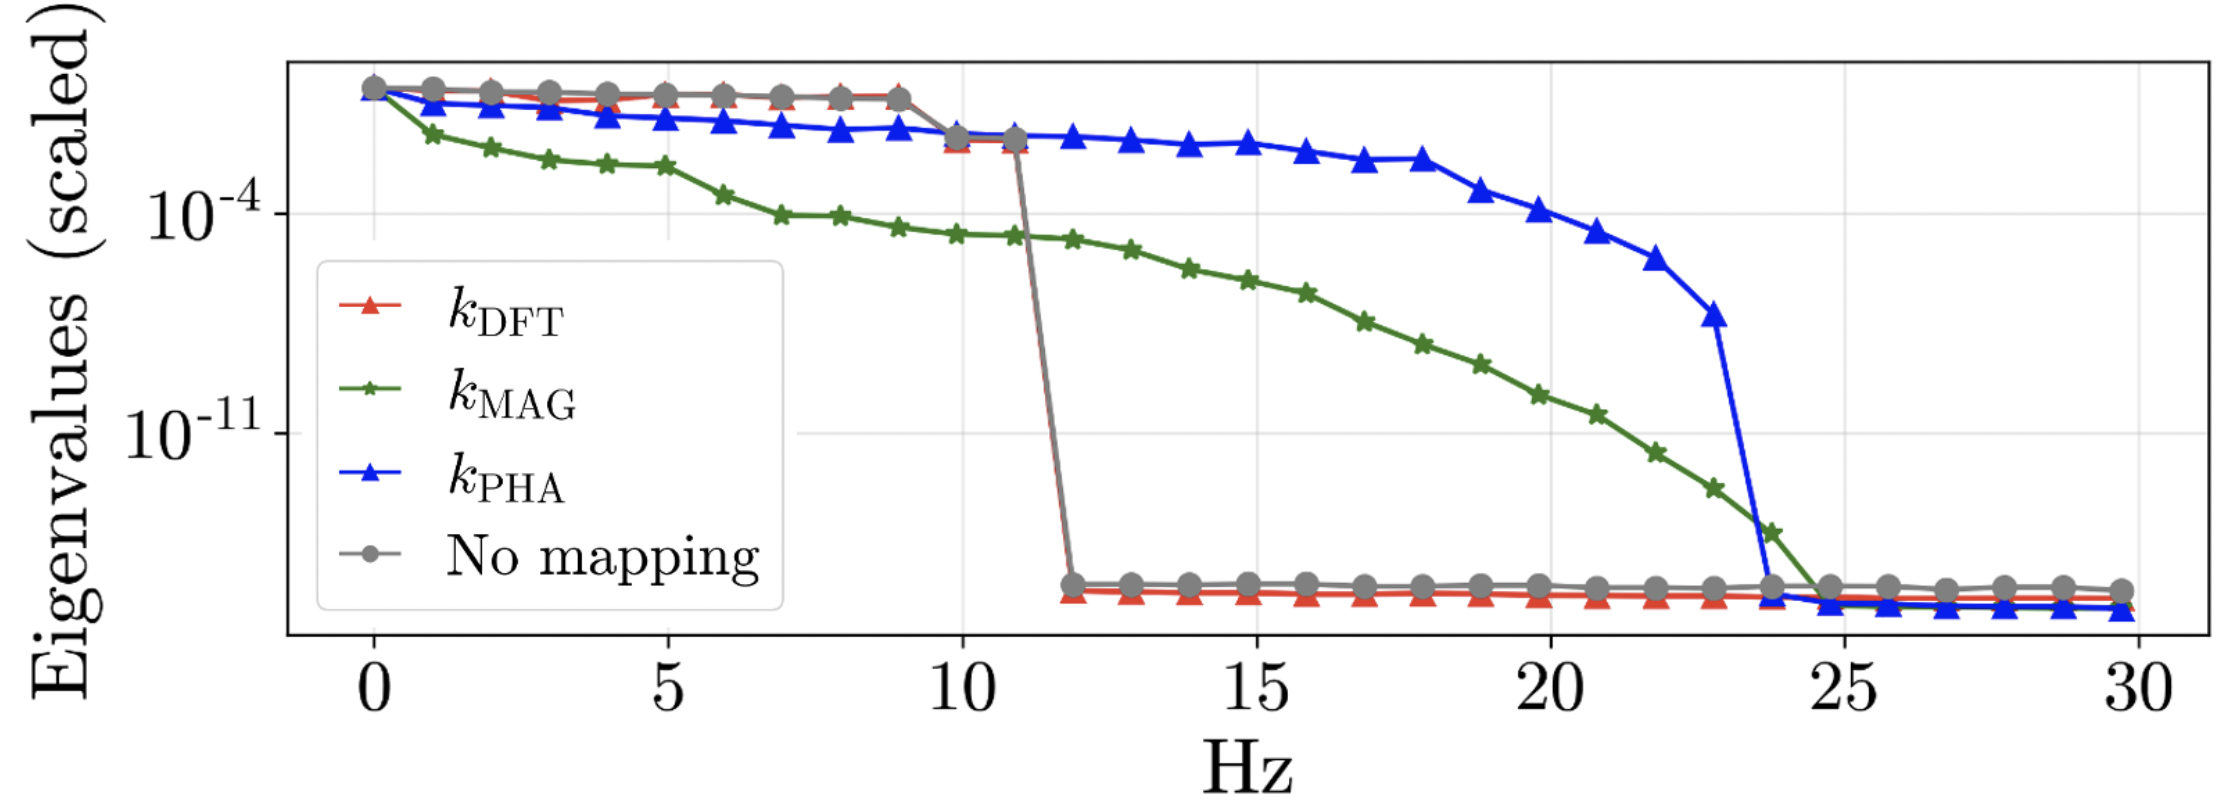
\includegraphics[width=0.4\textwidth]{eigenvalues}
  \caption{Kernel spatial of the kernel matrices}
  \label{fig:eigenvalues}
\end{figure}
\\
\textbf{The physics simulator.} The core of the physics simulator is a neural ordinary differential equation (ODE). Neural ODE~\cite{NEURIPS2018_69386f6b} is a type of neural network (NN) models, where instead of specifying a discrete sequence of hidden layers, the derivative of the hidden state is parameterized using a NN.\@ Given the initial state ${\tilde{x}_{s}}$ predicted by the encoder and physical parameters ${\theta}$ predicted by the estimator, the ODE solver rollouts state trajectories ${\hat{x}_s}$~(\ref{eq:ode_solver}).
\begin{align}
  \label{eq:ode_solver}
  & \{ \hat{x}_s \}_{s=t-\tau+1}^{t} : \hat{x}_{t-\tau+1}, \ldots, \hat{x}_{t-1}, \hat{x}_t \nonumber \\
  & = \text{ODESolver}( \tilde{x}_{t-\tau+1}, \dot{x} = A({\theta}) x + B({\theta}) u, \tau, \triangle ),
\end{align}
where ${\triangle}$ is a sampling start interval.
\\
\textbf{The decoder network.} Depending on the type of the input observations — images or sensor measurements — the decoder network is either a deconvolutional or a feedforward network, that generates a reconstructed observation ${\hat{o}_s}$ from each of the states ${\hat{x}_s}$, simulated by the ODE solver.
\\
\textbf{The loss function.} The loss function consists of three loses~(\ref{eq:loss_function}). Firstly, the variational autoencoder (VAE) loss is used to train the encoder ${h}$, the estimator ${f}$ and the decoder ${g}$. Secondly, the observation reconstruction loss used to minimize the error between input ${o_s}$ and reconstructed ${\hat{o}_s}$ observations, which improves the image reconstruction quality. Thirdly, the state reconstruction loss encourages states, defined by encoder ${\tilde{x}_{s}}$ to follow the ones, generated by physics simulator ${\hat{x}_s}$ and constrains the encoder from predicting arbitrary sequences.
\begin{equation}
  \label{eq:loss_function}
  \begin{aligned}
  L &= \sum_{s=t-\tau+1}^{t} D_{KL}(Q(\tilde{x}_s|o_s) || P(\tilde{x}_s)) \\
  &\quad + \sum_{s=t-\tau+1}^{t} \| o_s - \hat{o}_s \|_2^2 + \sum_{s=t-\tau+1}^{t} \| \tilde{x}_s - \hat{x}_s \|_2^2
  \end{aligned}
\end{equation}
\section{Performance Evaluation}
\section{ALPS Limitations}
A Impact of ALPS (and assumptions)
\section{Future Work}
We think the future extension
of ALPS to differentiable rendering engines is a valuable future research direction.
\\
We see that the network mostly uses the observation in the beginning and the end of the attention
mask to infer states. This suggests that the network learns to predict an average velocity. In addition,
we see that there are vertical attention patterns, which happens to be at the peak of the cosine wave.
We suspect that the network uses this information as an anchor to capture the periodic behavior of the
pendulum. We leave this as a future work to understand the network.
\section{Conclusions}

\begin{screenonly}
\subsection{This is an example of Appendix subsection head}

Channel-switching time is measured as the time length it takes for
motes to successfully switch from one channel to another. This
parameter impacts the maximum network throughput, because motes
cannot receive or send any packet during this period of time, and it
also affects the efficiency of toggle snooping in MMSN, where motes
need to sense through channels rapidly.

By repeating experiments 100 times, we get the average
channel-switching time of Micaz motes: 24.3 $\mu$s. We then conduct
the same experiments with different Micaz motes, as well as
experiments with the transmitter switching from Channel 11 to other
channels. In both scenarios, the channel-switching time does not have
obvious changes. (In our experiments, all values are in the range of
23.6 $\mu$s to 24.9 $\mu$s.)

\subsection{Appendix subsection head}

The primary consumer of energy in WSNs is idle listening. The key to
reduce idle listening is executing low duty-cycle on nodes. Two
primary approaches are considered in controlling duty-cycles in the
MAC layer.
  
\end{screenonly}

% Bibliography
\bibliographystyle{ACM-Reference-Format}
\bibliography{learning-physics}

\end{document}
